\documentclass[letterpaper,10pt,conference]{ieeeconf}
\IEEEoverridecommandlockouts
\overrideIEEEmargins

\usepackage{amsmath,amssymb}
\usepackage{booktabs}
\usepackage{graphicx}
\usepackage{url}
\usepackage{flushend}

\title{Earning a Dynamics Claim:\\
An Execution-Grounded Admission Audit for Robot Action Verification}

\author{Anonymous Authors}

\begin{document}
\maketitle
\thispagestyle{empty}
\pagestyle{empty}

\begin{abstract}
Dynamic robot-action benchmarks should earn a dynamics interpretation: high
verification accuracy may instead arise from current geometry, action
templates, unordered motion, or a short history suffix. We formulate
benchmark admission as an execution-grounded intervention with three gates.
Integrity ties labels to candidate executions under a declared observable
contract; temporal necessity progressively removes named shortcut routes; and
method headroom requires comparison to the strongest fair analytic or
geometric control. Our controlled state-observation identification test uses 92,000
GPU-PhysX candidate executions,
matched final observations and final-two-frame suffixes, action-diverse sets,
and three independent out-of-distribution axes. A lightweight GRU obtains
1.000 pair-order accuracy, exceeding the validation-selected fair analytic
estimator by 0.400 (base-world-clustered 95\% interval [0.3767, 0.4217]). On a
pinned public WAV MiniGrid split, paired evidence beats the strongest
single-state control by 0.459--0.476 dynamic accuracy across five state
complexities, while the released SparseIDM scores 0.940--0.953. The same audit
rejects learned-method headroom in an RGB-D stress test because fair centroid
velocity reaches 1.000 pair-order in all three families. It also rejects
alternate chunks in public real-UR5 logs because they lack matched physical
re-execution, despite a 0.950 standard-baseline test score. The contribution is
an auditable admit-or-reject procedure, not a claim of general visual
reasoning, real-robot transfer, or safety.
\end{abstract}

\section{Introduction}

Robot learning systems are increasingly evaluated on tasks described as
dynamic, from broad simulated manipulation suites to visual real-robot control
\cite{james2019rlbench,brohan2022rt1,nasiriany2024robocasa}. Yet a dynamic
label need not require a dynamic decision rule. If current geometry, an action
index, or an unordered set of observations predicts success, a verifier can
score highly without using temporal direction. Matching only the final
observation is also insufficient: a method may exploit aggregate displacement
or the last two frames.

This distinction matters for candidate-action verification. A verifier is
often used as a critic, reranker, or safety-adjacent filter, so benchmark
performance is easily interpreted as evidence that it understands how a scene
will evolve. Recent systems explicitly use interaction history or spatial
reasoning to select among generated robot actions
\cite{li2025have,zhao2026verispace}. That interpretation is warranted only when
simpler observable routes have been excluded and outcomes remain tied to the candidate action.
Benchmark validity and benchmark hardness are separate questions: a task can
have clean splits and still be saturated by a fair analytic control.

We treat this as a benchmark-admission problem. The unit of intervention is
the interpretation licensed by a benchmark, not a new verifier prediction.
An execution-grounded counterfactual audit constructs paired histories that
retain prescribed observable information while candidate executions yield
different outcomes. A progressive ladder tests static, action-template,
order-invariant, final-two-frame, and candidate-degeneracy shortcuts. The
result is deliberately asymmetric: passing can authorize a dynamics
comparison, while any failed gate rejects only the corresponding claim. In
particular, a learned-method claim is not authorized when a simple fair
estimator closes the intended headroom.

Our contributions are:
\begin{itemize}
    \item a three-gate admission intervention---integrity, temporal necessity,
    and method headroom---with an explicit observable contract, progressive
    counterfactual ladder, and refusal rule for unsupported method claims;
    \item the controlled \textsc{TimeArrow} identification test: 92,000
    execution-derived labels, an exact early-history pair swap, action-diverse
    C5/C10/C20 ranking, grouped splits, three OOD axes, leakage audits, and
    clustered uncertainty;
    \item a preregistered public WAV MiniGrid audit that confirms transition
    necessity across five state complexities without claiming a new method;
    \item two diagnostic rejections: a matched RGB-D construction whose fair
    geometric control saturates pair ordering, and public real-UR5 logs whose
    alternate chunks lack matched physical re-execution.
\end{itemize}

The central contribution is the evaluation intervention rather than the GRU.
We deliberately bound every conclusion to the named procedural families and
observations.

\section{Related Work}

Large robot policies and simulation suites emphasize breadth of control and
generalization \cite{brohan2022rt1,james2019rlbench,nasiriany2024robocasa};
our question is narrower and complementary: does an action verifier use the
temporal evidence its benchmark is intended to test? Visual foresight and
world-model methods predict action-conditioned futures for control
\cite{ebert2018visualforesight,hafner2023dreamerv3}, whereas we neither learn a
visual future model nor claim policy improvement.

History-aware verifiers rank candidates using past physical interactions
\cite{li2025have}, spatially grounded verifiers target geometric validity and
goal progress \cite{zhao2026verispace}, and World Action Verifier separates
state plausibility from action reachability to improve world models
\cite{liu2026wav}. These works design stronger verification mechanisms. We
instead audit whether a controlled verifier benchmark identifies the evidence
that its interpretation requires. We also apply our evidence controls to WAV's
public MiniGrid inverse-dynamics split; the result concerns that frozen
benchmark only, not a competing verifier architecture or WAV's robot results.

Shortcut learning describes decision rules that perform well for unintended
reasons \cite{geirhos2020shortcut,lapuschkin2019cleverhans}; causal confusion
has also been documented in imitation learning \cite{dehaan2019causal}.
Recent robot-policy studies connect shortcuts to dataset diversity and
fragmentation \cite{xing2025shortcut}, while LIBERO-CF counterfactually varies
language intent under plausible visual layouts \cite{fang2026liberocf}. Our
intervention instead matches candidate actions, current state, and the final
history suffix while deriving differing outcomes from execution.
Invariance and counterfactual methods motivate controlled comparisons across
environments \cite{arjovsky2019irm,wachter2017counterfactual}. Temporal-order
verification and arrow-of-time recognition learn video representations from
ordering cues \cite{misra2016shuffle,wei2018arrow}; unlike them, we ask whether
an action-conditioned evaluation actually requires those cues. PHYRE evaluates
physical reasoning in controlled environments \cite{bakhtin2019phyre},
CausalWorld exposes controllable factors in manipulation
\cite{ahmed2020causalworld}, and ManiSkill supplies GPU-parallel simulation and
rendering \cite{tao2024maniskill3}. We contribute an admission audit specialized
to candidate-action verification: observable matching, execution-derived
outcomes, action-diversity gates, and fair-estimator saturation checks.
The public ASU TableTop data provide real UR5 language-conditioned
manipulation trajectories \cite{zhou2023modularity}; we use them only to test
whether a logged formulation qualifies for stronger causal interpretation.

\section{Benchmark Admission as an Intervention}

\subsection{Verification task}

For world $w$, let $H=(o_1,\ldots,o_L)$ be an ordered observable history,
$A_w$ a candidate set, and $a\in A_w$ a candidate action. Executing $a$ in
the simulator produces $Y_w(a)\in\{0,1\}$ under one common success rule. A
verifier produces a score $s(H,a)$ used both to order a matched positive and
negative example and to rank candidates within a world.

Fair inputs may contain timestamped observations, visibility or confidence,
the robot TCP state, and the candidate action. They exclude family,
mechanism, branch, object identity, future trajectory, and outcome fields. A
counterfactual group contains members whose frozen observable constraints
match but whose execution outcomes differ. Pair-order accuracy gives one for
correct strict ordering, zero for reversed ordering, and the frozen tie value
otherwise. Candidate Top-1 evaluates $Y_w(\arg\max_a s(H,a))$; it is a
different estimand and is always reported separately.

\subsection{Progressive shortcut ladder}

Figure~\ref{fig:audit} summarizes the audit. Stage I measures shortcut-heavy
ordinary data. Stage II matches current geometry and candidate fields. Stage
III additionally matches unordered history statistics while changing signed
temporal direction. Stage IV matches the final two frames and changes only
earlier branch-identifying history. Stage V requires action-diverse candidate
sets and independent OOD cells.

\begin{figure*}[t]
    \centering
    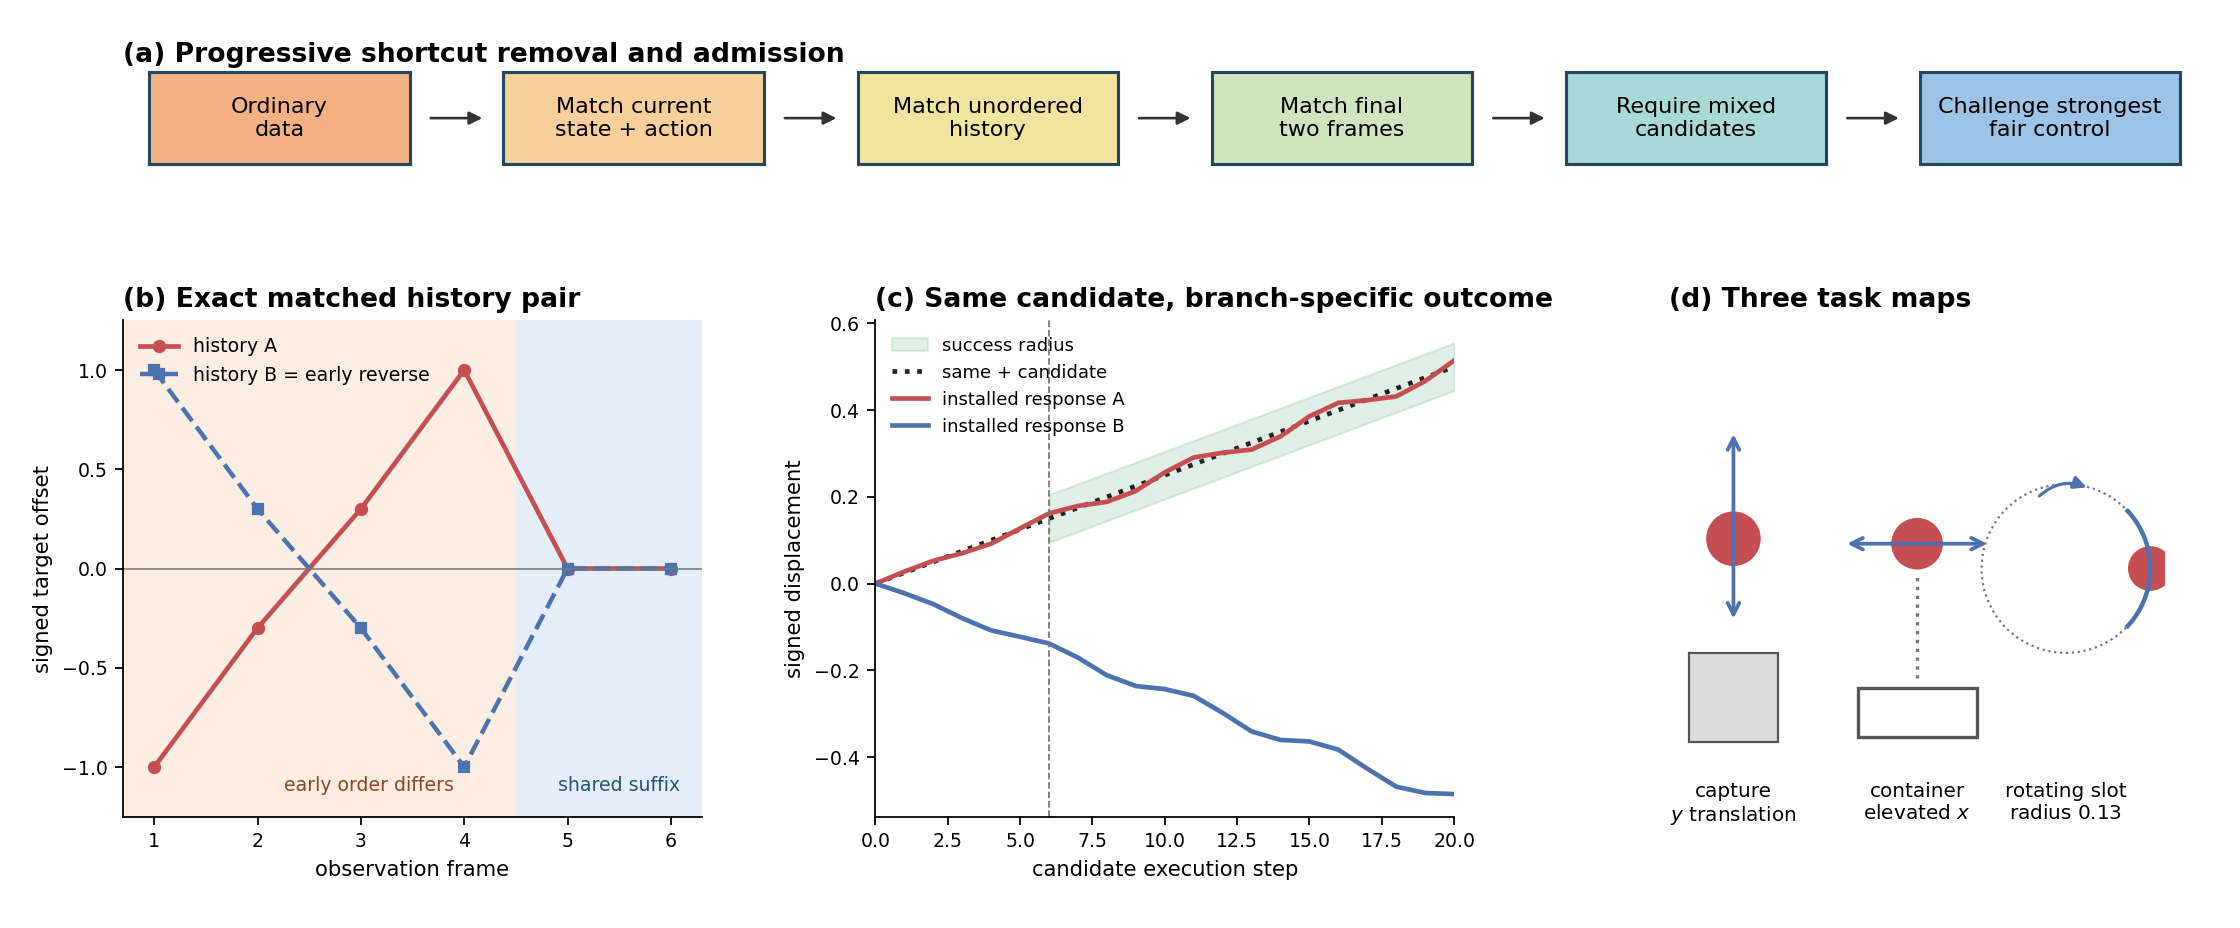
\includegraphics[width=0.98\textwidth]{figures/state_audit_construction.png}
    \caption{Audit and state construction. (a) Each stage removes one named
    shortcut before testing headroom. (b) One history is the exact early-frame
    reverse of its partner and both share the final suffix. (c) An illustrative
    ID damping/drive world: the same positive-direction candidate falls within
    the 0.055 success band for one installed response but not the other after
    the step-6 evaluation onset. (d) The three task families map the response
    to distinct geometry.}
    \label{fig:audit}
\end{figure*}

For six-frame histories, our final observable swap is
\begin{equation}
T(H)=\bigl(\operatorname{reverse}(H_{1:4}), H_{5:6}\bigr).
\end{equation}
It maps each generated partner exactly while retaining the two common
synchronization frames. A generic reversal is not a valid intervention because
it moves these frames and changes timestamp alignment; we retain it only as a
diagnostic. The pair-swap test evaluates $s(T(H),a)$ against the known partner,
and score-swap consistency checks whether paired scores exchange as intended.

Table~\ref{tab:contract} makes the tested threat model explicit. Each row
removes one route while retaining the information needed by later rows. This
ordering prevents a chance static score from being mistaken for temporal
necessity when a last-two-frame or geometric rule remains perfect.

\begin{table}[t]
    \centering
    \caption{Observable contract and corresponding rejection test.}
    \label{tab:contract}
    \resizebox{\columnwidth}{!}{%
    \begin{tabular}{lll}
        \toprule
        Threat & Preserved or matched & Rejection test \\
        \midrule
        Current-state cue & $o_6$, $a$, TCP & Static/current model \\
        Action template & Same $a$ across pair & Action-only model \\
        Orderless motion & Early-history multiset & Unordered model \\
        Short suffix & Exact $o_{5:6}$ & Final-two estimator \\
        Candidate degeneracy & Mixed C5/C10/C20 & Top-1 + diversity \\
        Hidden identity & Grouped worlds, whitelist & Leakage audit \\
        Analytic saturation & All legal geometry & Strongest fair rule \\
        \bottomrule
    \end{tabular}}
\end{table}

\subsection{Benchmark-admission rule}

We distinguish three gates. \emph{Validity} requires exact matching, grouped
split containment, hidden-field exclusion, common label semantics, mixed
candidate outcomes, and no candidate-index/template shortcut. \emph{Temporal
necessity} requires static, order-invariant, and final-two controls to fail on
the intended pair distinction. \emph{Method headroom} requires the strongest
fair analytic or geometric estimator to remain below the relevant oracle or
temporal comparator. Writing the gates as $G_V,G_T,G_H$, a temporal
interpretation requires $G_V\wedge G_T$, whereas a learned-method comparison
requires $G_V\wedge G_T\wedge G_H$. A failed gate is an audit result rather
than a missing experiment; no gate provides a safety guarantee.

\section{Controlled Identification Benchmark}

\subsection{Construction and labels}

\textsc{TimeArrow} is an identification test, not a surrogate for natural
robot data. It contains damped moving capture, hysteretic moving container,
and damped rotating-slot families with history-identifiable damping/drive and
hysteretic mode memory. Each label is obtained by a
GPU-PhysX proxy-to-target execution, using a common interception radius of
0.055 over execution steps 6--20. The analytic formulas used by fair baselines
do not produce labels.

For transparency, the post-decision target motion is procedural. With branch
$b\in\{0,1\}$, sign $\sigma_b=(-1)^b$, and execution step $n$, the two frozen
responses are
\begin{align}
d_b^{\mathrm{drv}}(n)&=\sigma_b\!\left[0.025n+0.020(1-e^{-\lambda n})
\sin(\omega n+\pi b)\right],\\
d_b^{\mathrm{hys}}(n)&=0.001\sigma_b[n-\delta_b]_+^2.
\end{align}
The three families map $d_b$ to translation along $y$, translation along $x$
at a fixed elevated goal, or angular motion on a 0.13-radius circle. At each
simulator step the target pose is updated by this rule and the candidate moves
a kinematic TCP proxy; the recorded label is the monotone OR of the scene's
distance-based success output, never an analytic-baseline prediction.

The observation histories are also controlled rather than natural rollouts.
Their first four target offsets are $[-s,-\rho s,\rho s,s]$ for one branch and
the exact reverse for the other ($\rho=0.30$ or $0.36$); both then receive two
identical synchronized decision poses. This makes the intended evidence and
the exact intervention inspectable: earlier order identifies which frozen
post-decision response is installed, while the current state and candidate are
identical.

The final protocol uses five active family--mechanism ID cells, 300 ID worlds
per cell, 100 worlds per active OOD cell, and aligned C5/C10/C20 candidate
views. C20 contains ten candidates from each temporal direction; endpoint,
pulse time, and amplitude vary by template. ID therefore contains 1,500 base
worlds, two histories per world, 20 candidates per history, 60,000 labeled
examples, and 30,000 matched pairs. The modulo-five world split yields
36,000/12,000/12,000 train/validation/test examples without dividing a world
or pair. Across ID and independently generated OOD cells the frozen simulator
budget is 92,000 candidate executions; this is execution accounting, not a
claim of 92,000 independent worlds.

The physical OOD moves damping from $[0.12,0.18]$ to $[0.26,0.32]$ and drive
frequency from $[1.15,1.45]$ to $[1.85,2.15]$. Delay OOD moves response onset
from 0--1 to 2--3 steps. Held-mechanism OOD fits only damping/drive rows and
tests fresh hysteretic-mode worlds. These axes are procedural and disjoint by
construction; they do not approximate open-world or sim-to-real shift.

\subsection{Comparators and metrics}

Each state example exposes a six-by-20 observation history, timestamp,
visibility and confidence per frame, a 20-by-3 candidate trajectory, and the
three-dimensional TCP state. Shortcut controls include static MLP,
action-only, unordered-history MLP, and final-two finite difference. Fair
analytic estimators include
multi-frame and robust linear velocity, constant acceleration, exponential
smoothing, and Kalman-style filters. Learned diagnostics include a lightweight
GRU, temporal convolution, and ordered/unordered MLPs. Hidden state and oracle
features are excluded from the fair comparison.

The selected GRU has 8,577 parameters: a 32-unit recurrent state followed by a
32-unit action-conditioned head. AdamW uses learning rate 0.015; the selection
run uses three seeds and 100 full-batch updates. After validation-only model
and analytic-baseline selection, the confirmation run uses five fixed seeds
and 120 updates. Reported confirmation scores average logits across seeds.

The primary metric is pair-order accuracy. We additionally report Top-1,
Top-3 success recall, utility-gain NDCG, normalized regret, swap controls, and
inference latency. ID test contains 6,000 candidate-specific matched groups
nested in 300 base worlds. The paired interval first averages the 20
candidate-pair differences within each world, then resamples the 300 worlds
with 4,000 bootstrap draws (seed 7301). It characterizes variation over these
frozen procedural worlds, not an open-world population. Ties receive 0.5
throughout.

\section{State Results}

Validation selects GRU and MultiFrameLinearVelocity. Table~\ref{tab:state}
shows the frozen test comparison. GRU reaches 1.000 ID pair-order versus 0.600
for the fair analytic estimator, a +0.400 difference with base-world-clustered
95\% interval [0.3767, 0.4217]. The advantage remains positive under physical-parameter,
delay, and held-mechanism OOD; the weaker held-mechanism score (0.787) is
reported rather than hidden. ID uses validation selection for both sides. For
each OOD row we instead report the strongest fair analytic rule in that test
cell, an intentionally conservative oracle-control comparison rather than a
deployable selection procedure.

\begin{table}[t]
    \centering
    \caption{State pair-order accuracy. The analytic method is selected on
    validation for ID; each OOD row reports its frozen best fair analytic
    comparator.}
    \label{tab:state}
    \resizebox{\columnwidth}{!}{\begin{tabular}{lccc}
\toprule
Split & GRU & Fair analytic & $\Delta$ \\
\midrule
ID & 1.000 & 0.600 & +0.400 \\
Physical OOD & 1.000 & 0.500 & +0.500 \\
Delay OOD & 1.000 & 0.857 & +0.143 \\
Held mechanism & 0.787 & 0.667 & +0.120 \\
\bottomrule
\end{tabular}
}
\end{table}

Table~\ref{tab:state_diagnostics}(a) reports every analytic and learned ID
comparison, not only the winners. The three-seed ordered MLP reaches 0.900 and
the selection-run GRU reaches 0.985 on test, showing that the signal is not
unique to one confirmation run. Conversely, temporal convolution remains at
0.500; an architecture's failure is not evidence that the cue is absent.
Panel (b) exposes heterogeneity: the strongest analytic control saturates the
rotating-slot/hysteresis cell at 1.000, while it is at 0.500 in the other four
cells. Our aggregate claim therefore does not assert learned headroom in every
family--mechanism cell.

Candidate selection groups candidates by family, mechanism, world, and branch:
exactly one observable history. We explicitly reject the tempting but invalid
key that pools both counterfactual branches.
All 600 test histories at each candidate-set size contain both outcomes.
Panel (c) uses independently saved raw scores: GRU Top-1 is 1.000 at
C5/C10/C20, whereas static and action controls are 0.500. This history-key
audit leaves pair-order and OOD values unchanged.

\begin{table*}[t]
    \centering
    \begin{minipage}[t]{0.53\textwidth}
        \centering
        \textbf{(a) Complete ID comparison}\par\smallskip
        \resizebox{\linewidth}{!}{\begin{tabular}{lccc}
\toprule
Category & Method & Val. & Test \\
\midrule
Analytic & Last-two finite difference & 0.500 & 0.500 \\
Analytic & Multi-frame linear velocity & 0.600 & 0.600 \\
Analytic & Robust linear velocity & 0.600 & 0.600 \\
Analytic & Constant-acceleration fit & 0.400 & 0.400 \\
Analytic & Alpha--beta filter & 0.600 & 0.600 \\
Analytic & Kalman constant velocity & 0.600 & 0.600 \\
Analytic & Kalman constant acceleration & 0.600 & 0.600 \\
Analytic & Exponential smoothing & 0.400 & 0.400 \\
Learned (3) & Static MLP & 0.500 & 0.500 \\
Learned (3) & Action-only MLP & 0.500 & 0.500 \\
Learned (3) & Unordered-history MLP & 0.500 & 0.500 \\
Learned (3) & Temporal convolution & 0.500 & 0.500 \\
Learned (3) & Ordered temporal MLP & 0.900 & 0.900 \\
Learned (3) & GRU selection run & 0.987 & 0.985 \\
Confirm. (5) & GRU confirmation & 1.000 & 1.000 \\
\bottomrule
\end{tabular}
}
    \end{minipage}\hfill
    \begin{minipage}[t]{0.44\textwidth}
        \centering
        \textbf{(b) Frozen ID test cells}\par\smallskip
        \resizebox{\linewidth}{!}{\begin{tabular}{lcccc}
\toprule
Family & Mechanism & GRU & Strongest analytic & Score \\
\midrule
Damped capture & Damping/drive & 1.000 & Last-two FD & 0.500 \\
Damped capture & Hysteresis & 1.000 & Last-two FD & 0.500 \\
Rotating slot & Hysteresis & 1.000 & Multi-frame linear & 1.000 \\
Moving container & Damping/drive & 1.000 & Last-two FD & 0.500 \\
Moving container & Hysteresis & 1.000 & Last-two FD & 0.500 \\
\bottomrule
\end{tabular}
}
        \vspace{1.0em}

        \textbf{(c) History-keyed candidate ranking}\par\smallskip
        \resizebox{\linewidth}{!}{\begin{tabular}{lccccccc}
\toprule
Set & Contexts & Mixed & GRU Top-1 & Static & Action & NDCG & Regret \\
\midrule
C5 & 600 & 1.000 & 1.000 & 0.500 & 0.500 & 1.000 & 0.000 \\
C10 & 600 & 1.000 & 1.000 & 0.500 & 0.500 & 1.000 & 0.000 \\
C20 & 600 & 1.000 & 1.000 & 0.500 & 0.500 & 1.000 & 0.000 \\
\bottomrule
\end{tabular}
}
        \vspace{1.0em}

        \textbf{(d) Validity and temporal-necessity controls}\par\smallskip
        \resizebox{0.78\linewidth}{!}{\begin{tabular}{lc}
\toprule
Audit & Pair-order / rate \\
\midrule
Correct history & 1.000 \\
Final two only & 0.500 \\
Valid pair swap & 1.000 \\
Score-swap consistency & 1.000 \\
Nondegenerate C20 worlds & 1.000 \\
C20 dynamic Top-1 & 1.000 \\
\bottomrule
\end{tabular}
}
    \end{minipage}
    \caption{State diagnostics. Parenthetical counts in (a) are seeds.
    Cell-wise analytic rules in (b) are strongest-in-cell stress controls, not
    test-selected deployable models. ``Mixed'' in (c) is the fraction of
    history contexts containing both outcomes. Panel (d) reports final audit
    gates.}
    \label{tab:state_diagnostics}
\end{table*}

The controls in Table~\ref{tab:state_diagnostics}(d) support the intended interpretation.
Correct history is perfect while final-two-only is chance, so the result needs
earlier observations. The exact pair swap and score-swap consistency are both
1.000. Applying the exact early swap while retaining original labels reverses
the ordering completely (0.000); a generic full reversal remains at 0.982 and
is therefore not a valid causal test. All C20 worlds are nondegenerate, every branch changes at least one
candidate outcome, candidate-template success rates are balanced, and maximum
candidate-index leakage is zero. C20 p95 inference latency is 0.816 ms on the
recorded GPU. A red-team audit reports no blocking finding. Its one warning
records a bookkeeping correction to the C20 diversity audit; no simulator,
label, or score changed. The final history-key ranking correction is likewise
versioned and retains all 14 score arrays for independent recomputation.

Perfect pair scores should be read as controlled diagnostic separation, not as
evidence of universal physical reasoning. This is also why we next apply the
admission audit to visual observations instead of immediately proposing a
larger verifier.

\section{Benchmark-Admission Stress Tests}

\subsection{Public WAV MiniGrid transition check}

We first apply the audit to an established public verifier benchmark. WAV
releases a MiniGrid state-complexity split in which a model infers one of seven
actions from $(s_t,s_{t+1})$ and carried-object state \cite{liu2026wav}. Its
official dynamic-accuracy metric executes the predicted action with a public
physics oracle and scores only channels that changed in the logged transition;
it can therefore credit distinct actions with the same physical outcome. We
pin upstream commit \texttt{527159b}, its checkpoint, source, and six data-file
hashes. The official o6 training set has 2,000 transitions; untouched o6 and
o8/o10/o12/o14 tests contain 1,000 and 2,500 transitions, respectively.

Before training any control, we froze five seeds, a class-stratified 80/20
development split within o6, and three copies of one CNN architecture. The
current-only and next-only cells duplicate one state into both network slots;
the paired cell receives the unmodified transition. All use identical
optimization and validation action-accuracy selection. We separately evaluate
the released SparseIDM checkpoint over five inference seeds and a fixed
transition rule using agent pose, the front cell, and carried-object changes.
No test split selects a model or hyperparameter.

\begin{table*}[t]
    \centering
    \caption{External audit of the public WAV MiniGrid state-complexity split.
    Entries are official dynamic accuracy; learned cells and SparseIDM report
    mean$\pm$sample standard deviation over five seeds. ``Strongest single'' is
    the larger of the separately evaluated current-only and next-only means at
    each complexity. The transition rule has 1.000 action accuracy; its
    subunit dynamic score exposes the public oracle/log mismatch and is treated
    as an observed ceiling, not used to normalize other scores.}
    \label{tab:wav}
    \resizebox{0.94\textwidth}{!}{\begin{tabular}{lccccc}
\toprule
Objects & $N$ & Strongest single & Paired CNN & SparseIDM & Transition rule \\
\midrule
6 & 1000 & 0.410$\pm$0.024 & 0.879$\pm$0.012 & 0.947$\pm$0.000 & 0.947 \\
8 & 2500 & 0.378$\pm$0.052 & 0.853$\pm$0.020 & 0.953$\pm$0.000 & 0.958 \\
10 & 2500 & 0.329$\pm$0.047 & 0.805$\pm$0.044 & 0.940$\pm$0.001 & 0.952 \\
12 & 2500 & 0.343$\pm$0.042 & 0.811$\pm$0.043 & 0.951$\pm$0.001 & 0.962 \\
14 & 2500 & 0.341$\pm$0.083 & 0.800$\pm$0.041 & 0.947$\pm$0.002 & 0.969 \\
\bottomrule
\end{tabular}
}
\end{table*}

Table~\ref{tab:wav} passes all preregistered gates. Paired evidence improves
over the strongest single-state control by 0.469, 0.475, 0.476, 0.468, and
0.459 from o6 through o14. The released SparseIDM remains at 0.940--0.953, and
the transition rule exceeds every single-state control. This is positive
external evidence that the named inverse-dynamics benchmark requires the
observed state transition under our controls. It does not audit WAV's Action Following Score,
its robot setting, or real-robot verification.

\subsection{Visual RGB-D construction}

We construct a separately versioned visual pilot because exact RGB-D
reconstruction of the state histories cannot be established after the fact.
For each of three procedural families, it contains 128 base worlds, two matched
histories, ten shared candidate actions, six 128$\times$128 RGB-D frames, and
2,560 candidate executions (7,680 total). Pair members share current RGB,
depth, and action fields but differ in earlier history. Splits contain complete
world groups; segmentation, identifiers, branch, mechanism, and future fields
are excluded. The storage audit verifies exact current/final-two/action,
unordered-history, mask, and metadata matching; no malformed group is found.
Pair-label disagreement is 1.000 for moving cube/window and 0.974 for rotating
window, and pair-order uses only opposite-label pairs. The fraction of
histories with mixed C10 outcomes is 1.000, 1.000, and 0.977, respectively.

\begin{figure*}[t]
    \centering
    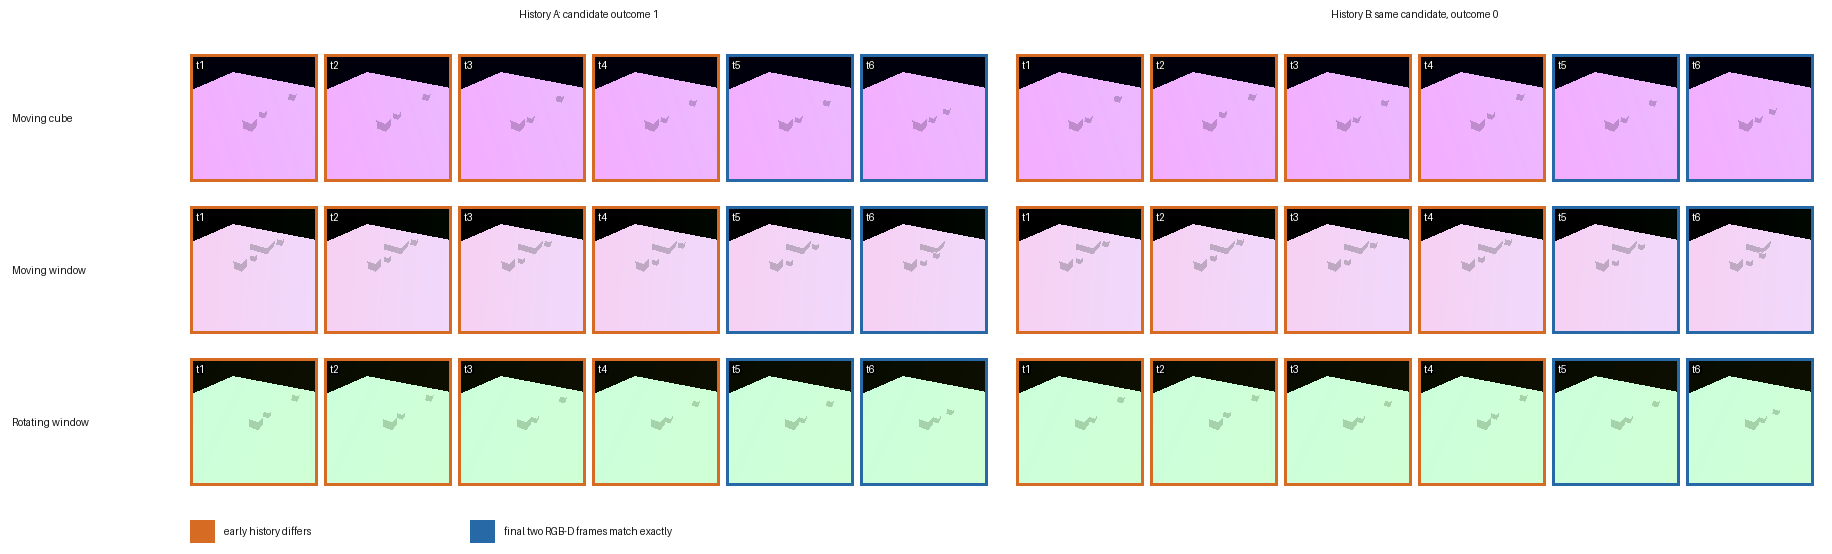
\includegraphics[width=\textwidth]{figures/visual_matched_histories.png}
    \caption{Audited complete-history examples from one held-camera test world.
    Orange frames contain the differing early history; blue frames are the
    exact common RGB-D suffix. For candidate slot 0, history A's execution
    succeeds and history B's fails in every displayed family. The montage is
    generated from frozen bundles after checking nine exact source hashes; RGB
    is shown, while equality is asserted for both RGB and depth.}
    \label{fig:visualpairs}
\end{figure*}

We use a held test camera and the union of ten non-complete conditions:
random/burst missing frames, asynchronous RGB or depth, missing final frame,
target occlusion, irregular timestamps, and latency. The frozen artifact calls
this regime \texttt{combined\_held\_dropout}; here we use the more precise term
\emph{held-camera + corruption}. RGB-D and depth-backprojected world points are
pooled deterministically from 128$\times$128 to 16$\times$16. Fair controls
include action-only, current and unordered observations, ordered RGB-D GRU,
world-frame point-cloud GRU, and a segmentation-free MLP over per-frame global
centroid, centroid difference, and speed. Calibration is legal input; target
masks and the separate oracle files are not. All learned visual controls use
seeds 17/29/43 and the same grouped fit split.

Table~\ref{tab:visual} gives three-seed point estimates. Action-only and
current RGB-D remain exactly at 0.500. Ordered RGB-D GRU reaches only
0.537--0.665, while world-frame point-cloud normalization improves this to
0.727--0.860. However, centroid velocity reaches 1.000 pair-order in all three
families, matching the clean-state oracle and leaving zero pair-order headroom.
Because this control pools every valid scene point rather than using object
identity, its success is itself a global-motion shortcut. The task therefore
passes integrity and temporal-necessity checks but fails method admission.

\begin{table*}[t]
    \centering
    \caption{Visual stress test under held-camera + corruption (the frozen
    \texttt{combined\_held\_dropout} key, all non-complete test histories).
    Columns except ``Cent. Top-1'' are pair-order accuracy. The frozen visual
    confidence intervals are intentionally suppressed because their score-
    ensemble bootstrap estimand does not match the displayed seed-average
    point estimate.}
    \label{tab:visual}
    \resizebox{0.87\textwidth}{!}{\begin{tabular}{lcccccc}
\toprule
Family & Action & Current & RGB-D & World-PC & Centroid & Cent. Top-1 \\
\midrule
Moving cube & 0.500 & 0.500 & 0.665 & 0.860 & 1.000 & 0.673 \\
Moving window & 0.500 & 0.500 & 0.537 & 0.727 & 1.000 & 0.653 \\
Rotating window & 0.500 & 0.500 & 0.569 & 0.767 & 1.000 & 0.727 \\
\bottomrule
\end{tabular}
}
\end{table*}

This negative decision reveals a second evaluation trap. Pair ordering and
C10 action selection are not interchangeable: although centroid pair-order is
1.000, its Top-1 success is only 0.653--0.727. A method paper could still study
multi-candidate ranking under a newly frozen protocol, but it cannot cite the
current paired task as unsolved learned-method headroom. The audit prevents a
post-hoc method claim instead of treating a stopped experiment as missing
evidence.

\subsection{Public real-robot log scope check}

We also apply the admission rule to a frozen formulation built from public ASU
TableTop UR5 logs \cite{zhou2023modularity}. It contains 84 episodes from 11
official action--object tasks and 1,151 C5 candidate sets. The harder split
trains on bread/bottle/cube, validates on Pepsi, and tests on unseen Coke/milk
goal objects using whole episodes. Action-, task-, language-, source-, and
shuffled-smoothness validation controls are at most 0.534, but a standard
proprio-action GRU reaches 0.972 validation and 0.950 test pair-order.

This does not establish counterfactual real-robot verification. The positive
is the actual next action chunk; the four negatives are distant, other-episode,
different-task, or reversed chunks drawn from existing logs. They were never
executed from the same decision state and therefore have no candidate-specific
physical outcomes. The audit consequently rejects the formulation at both
execution grounding and method headroom, before training a proposed verifier.

Table~\ref{tab:admission} makes the asymmetric outcome explicit. The controlled
state identification test and public WAV MiniGrid split pass their respective
temporal-evidence gates. The visual construction passes integrity and temporal-necessity
checks but loses all pair-order headroom to a fair geometric estimator; the
real-log task lacks matched re-execution. These negative cases are useful
evidence for the audit procedure precisely because they are rejected.

\begin{table*}[t]
    \centering
    \caption{Benchmark-admission decisions generated from the frozen reports.
    ``Integrity'' covers exact matching, grouped splits, hidden-field
    exclusion, and candidate diversity where applicable. State admission is
    an aggregate claim; one family--mechanism cell is analytically saturated.
    The WAV row covers only its MiniGrid inverse-dynamics split, and the UR5 row
    is logged-continuation identification, not matched re-execution.}
    \label{tab:admission}
    \resizebox{0.94\textwidth}{!}{\begin{tabular}{lcccc}
\toprule
Benchmark & Integrity & Temporal evidence & Fair-control test & Decision \\
\midrule
State observations & Pass & Final-two 0.500 & Analytic 0.600 vs GRU 1.000 & Admit controlled comparison \\
Public WAV MiniGrid & Pinned upstream & Single $\leq$0.356 & SparseIDM 0.948 & Admit transition evidence \\
Visual RGB-D stress test & Pass & Final-two 0.500; unordered $\leq$0.535 & Centroid 1.000 & Reject method claim \\
Public UR5 logs & Logged groups pass & Trivial val. $\leq$0.534 & Proprio GRU 0.972 val. & Reject: no re-execution \\
\bottomrule
\end{tabular}
}
\end{table*}

\section{Discussion and Limitations}

The state construction is procedural and simulator-specific. It uses clean
state observations, controlled TCP geometry, limited embodiment diversity,
and designed counterfactual factors. Its histories are instantiated from the
frozen response family rather than collected from unconstrained interaction;
the positive result therefore establishes diagnostic separation, not natural
dynamics fidelity. The visual stress test adds RGB-D,
occlusion/corruption, camera shift, and geometry extraction, but it is also
procedural and is explicitly rejected as a hard benchmark. Its backgrounds
and global scene motion make centroid saturation possible; adding visual
complexity without rerunning the admission ladder would not establish a fix.
The controlled experiments do not include language or contact-rich robot
outcomes. The public-log check adds language and real trajectories but still
lacks alternate-action robot executions. None includes end-to-end policy
learning or safety validation.

The external WAV check broadens benchmark provenance but not embodiment: it is
a discrete MiniGrid inverse-dynamics task, not the WAV Action Following Score
or robot experiment. Its public physics oracle does not exactly reproduce every
logged changed channel even for the true action, so the transition rule's
0.947--0.969 dynamic accuracy is an empirical ceiling rather than 1.000. This
does not affect the preregistered paired-versus-single comparison, but it limits
cross-metric interpretation.

Counterfactual language here is local to the frozen generator and exact swap;
we do not claim an intervention on arbitrary real videos. Execution grounding
separates the success label from analytic estimators, but does not by itself
eliminate simulator artifacts. The world-clustered state interval and visual
three-seed point estimates have different statistical units and are never
pooled. Finally, a benchmark that defeats the named controls may admit an
unknown shortcut; publishing the observable contract and admission tests is
therefore part of the contribution. Perfect state scores may also indicate
that the final procedural distinction is cleaner than natural dynamics. Future
work should apply the same ladder to matched real-robot re-executions; analytic
saturation would remain an informative rejection rather than missing evidence.

\section{Reproducibility and Conclusion}

A downstream-only builder reads sixteen frozen JSON reports, checks their exact
SHA-256 hashes plus the corrected-ranking raw-score hash, enforces 36
scientific invariants, suppresses the invalid visual CI, and deterministically
emits the paper tables and a claim ledger. No training or evaluator code is
imported during table generation. The ranking correction stores all five GRU
and six control-seed score vectors plus their means; a verify-only path
recomputes every history-keyed metric. The visual montage independently checks
nine bundle/candidate/label hashes and the exact RGB-D suffix. The package also
records split and leakage audits, execution accounting, and both non-blocking
bookkeeping fixes plus the world-clustered interval correction. The external
audit stores confusion counts and prediction hashes for every method, seed, and
complexity; an independent verifier recomputes all summaries and 15 frozen gates.

We conclude that dynamic labels and chance-level static controls are necessary
but insufficient evidence of temporal reasoning. Execution-grounded matched
pairs expose named shortcuts in the state setting, while the same admission
logic confirms transition necessity on a pinned public verifier split and
correctly rejects a visual construction saturated by simple geometry and a
real-log task without matched alternate-action outcomes.
This combination---positive controlled evidence and an explicit refusal to
claim headroom when it is absent---makes action-verifier evaluation more
falsifiable.

\section*{Acknowledgment}

OpenAI Codex was used to assist with drafting and revising the Abstract,
Introduction, Related Work, Discussion and Limitations, Reproducibility and
Conclusion, and this disclosure; implementing downstream audit and
verification code; and orchestrating execution of the frozen experiment
scripts. All reported observations were produced by those scripts from hashed
inputs; the authors verified the protocols, claims, source values, code, and
generated artifacts.

\bibliographystyle{IEEEtran}
\bibliography{references}

\end{document}
